\section{Prototype}
The overall functionalities for the project has been limited, due to time limitations and to focus on the scope of the project. In this project a prototype will therefore be made to show the main functionalities necessary to make a automated vehicle.
In short the final prototype is to contain a regulator which will make it possible to follow a path from A to B. It is be able to continue if the transmission is lost between the prototype and the GoT system for some duration. Furthermore it stores data points locally, on the vehicle, from the GoT system. The rough outline of the design is shown on \figref{fig:systemOverview1} to give an idea of the final prototype setup.

\begin{figure}[H]
	\centering
	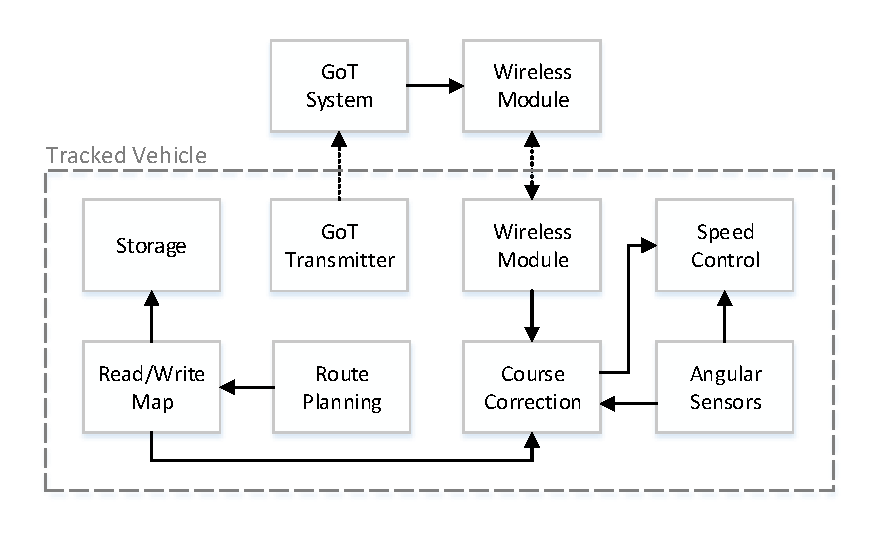
\includegraphics[scale=.9]{figures/systemOverview1}
	\caption{Overview of the system prototype}
	\label{fig:systemOverview1}
\end{figure}




\begin{figure}[H]
	\centering
	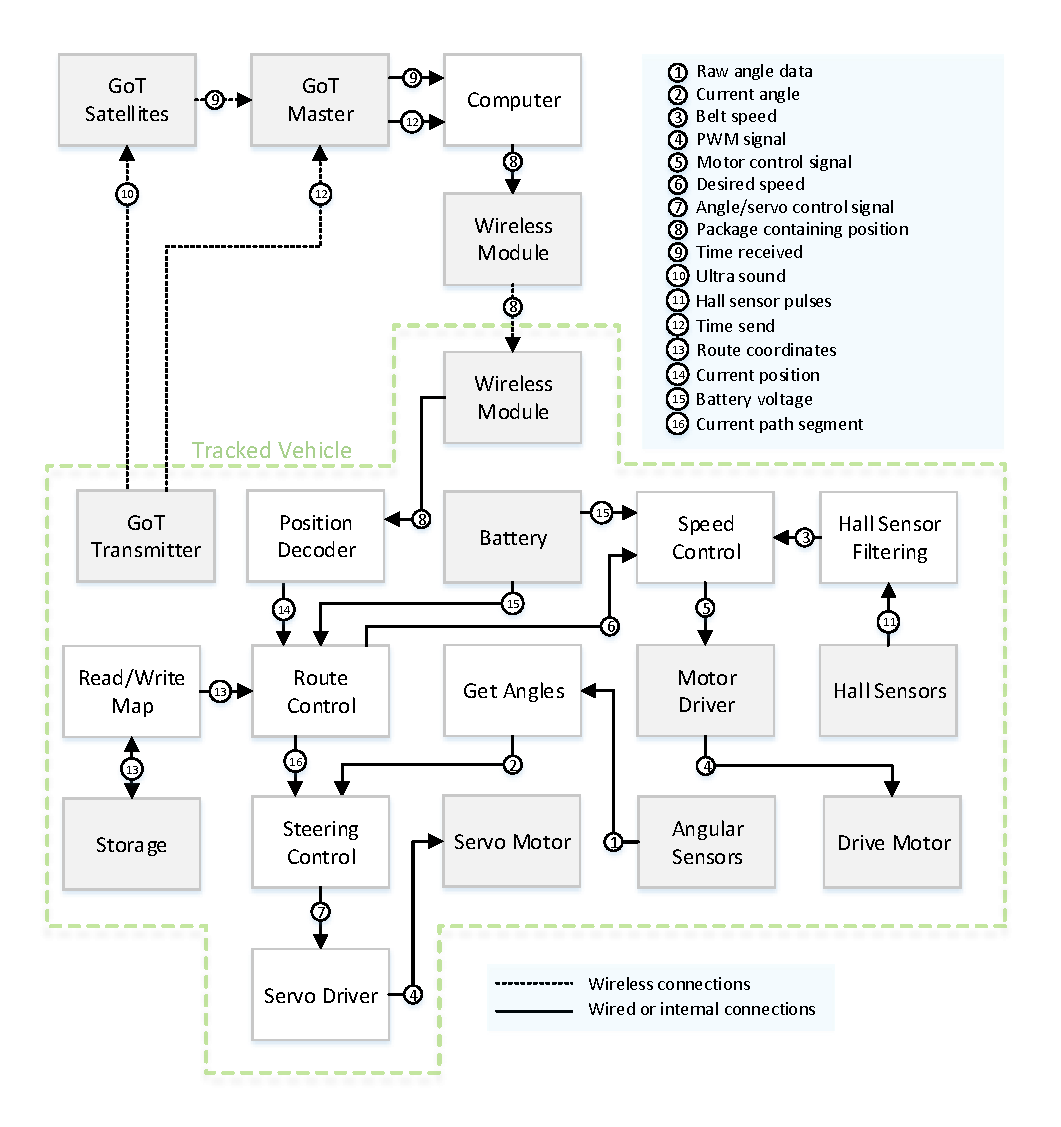
\includegraphics[scale=.9]{figures/systemOverview2}
	\caption{Expanded overview of the system prototype}
	\label{fig:systemOverview2}
\end{figure}